% STOLAR Data Descriptor
% Iver Raknes Finne, AHO, 2026
% Compile: pdflatex main && bibtex main && pdflatex main && pdflatex main
% ══════════════════════════════════════════════════════════════
% STOLAR Data Descriptor — two-column research publication format
% Matching foundational-paper style
% ══════════════════════════════════════════════════════════════

\documentclass[10pt, a4paper, twocolumn]{article}

% ── Encoding & fonts ──
\usepackage[T1]{fontenc}
\usepackage[utf8]{inputenc}
\usepackage{newtxtext}              % Times Roman
\usepackage{newtxmath}              % Matching math fonts
\usepackage[final]{microtype}       % Optical margin alignment

% ── Page geometry ──
\usepackage[
  top=20mm, bottom=22mm,
  left=16mm, right=16mm,
  columnsep=7mm,
  headsep=8mm, footskip=10mm
]{geometry}

% ── Line spacing ──
\usepackage{setspace}
\setstretch{1.12}
\setlength{\parskip}{0pt}
\setlength{\parindent}{1em}

% ── Section headings ──
\usepackage{titlesec}
\titleformat{\section}
  {\normalfont\large\bfseries}{\thesection.}{0.5em}{}
\titleformat{\subsection}
  {\normalfont\normalsize\bfseries}{\thesubsection.}{0.4em}{}
\titleformat{\subsubsection}
  {\normalfont\normalsize\itshape}{\thesubsubsection.}{0.4em}{}
\titlespacing*{\section}{0pt}{14pt plus 2pt minus 1pt}{5pt plus 1pt}
\titlespacing*{\subsection}{0pt}{8pt plus 2pt minus 1pt}{2pt plus 1pt}
\titlespacing*{\subsubsection}{0pt}{6pt plus 1pt}{2pt}

% ── Citations ──
\usepackage[numbers,sort&compress]{natbib}
\bibliographystyle{unsrtnat}
\renewcommand*{\bibfont}{\small}

% ── Math ──
\usepackage{amsmath}

% ── Figures & tables ──
\usepackage{graphicx}
\usepackage{float}
\usepackage{booktabs}
\usepackage{array}
\usepackage{tabularx}
\usepackage{caption}
\captionsetup{
  labelfont={bf, small},
  font={small},
  skip=4pt,
  belowskip=2pt,
  format=plain,
  justification=justified,
  singlelinecheck=false
}

% ── Lists ──
\usepackage{enumitem}
\setlist{nosep, leftmargin=1.5em, topsep=2pt}

% ── Cross-references ──
\usepackage[
  colorlinks=true,
  linkcolor=black,
  citecolor=blue!50!black,
  urlcolor=blue!60!black
]{hyperref}
\usepackage{siunitx}

% ── Running head ──
\usepackage{fancyhdr}
\pagestyle{fancy}
\fancyhf{}
\fancyhead[L]{\footnotesize\textsc{STOLAR: open geometrisk database}}
\fancyhead[R]{\footnotesize\thepage}
\renewcommand{\headrulewidth}{0.4pt}
\fancypagestyle{plain}{%
  \fancyhf{}
  \fancyfoot[C]{\footnotesize\thepage}
  \renewcommand{\headrulewidth}{0pt}
}

\graphicspath{{figures/}}


\begin{document}

% ── Title block ──────────────────────────────────────────────────────────────
\twocolumn[{%
\begin{@twocolumnfalse}
\vspace*{4mm}
{\raggedright
{\fontsize{22}{26}\selectfont\bfseries STOLAR: An Open Geometric Database of\\2\,048 European Chairs (1280--2024)\par}
\vspace{6pt}
\textit{Iver Raknes Finne}\\[2pt]
{\small\textit{Institutt for design, Arkitektur- og designh\o gskolen i Oslo (AHO)}\\
\texttt{iver.raknes.finne@stud.aho.no}\par}
\vspace{10pt}
\noindent\small\textbf{Abstract}\enspace
Design history has long relied on qualitative case studies of individual artefacts.
Quantitative morphometric approaches, routine in palaeontology and evolutionary biology since Raup (1966),
remain rare in the study of designed objects.
We present STOLAR, an open research database of 2\,048 European chairs spanning 1280--2024,
compiled from the collections of the Nasjonalmuseet (Oslo) and the Victoria and Albert Museum (London).
Each record includes up to 30 metadata fields with 99\% dimensional coverage,
a background-removed photograph, and an AI-generated 3D mesh.
From the 3D meshes we extract five geometric shape descriptors:
sphericity, fill ratio, inertia ratio, complexity, and convex hull volume.
Principal component analysis of the shape descriptors reveals that 60\% of geometric variation
is explained by two axes: a compactness/roundness axis (PC1, 35.5\%) and a mass/complexity axis (PC2, 24.5\%).
The database, 3D models, and all analysis code are released under the MIT licence.
\par\vspace{6pt}
\noindent\small\textbf{Keywords}\enspace morphospace, design history, shape grammar, 3D morphometrics, cultural evolution, chair design
\par\vspace{10pt}
\centering
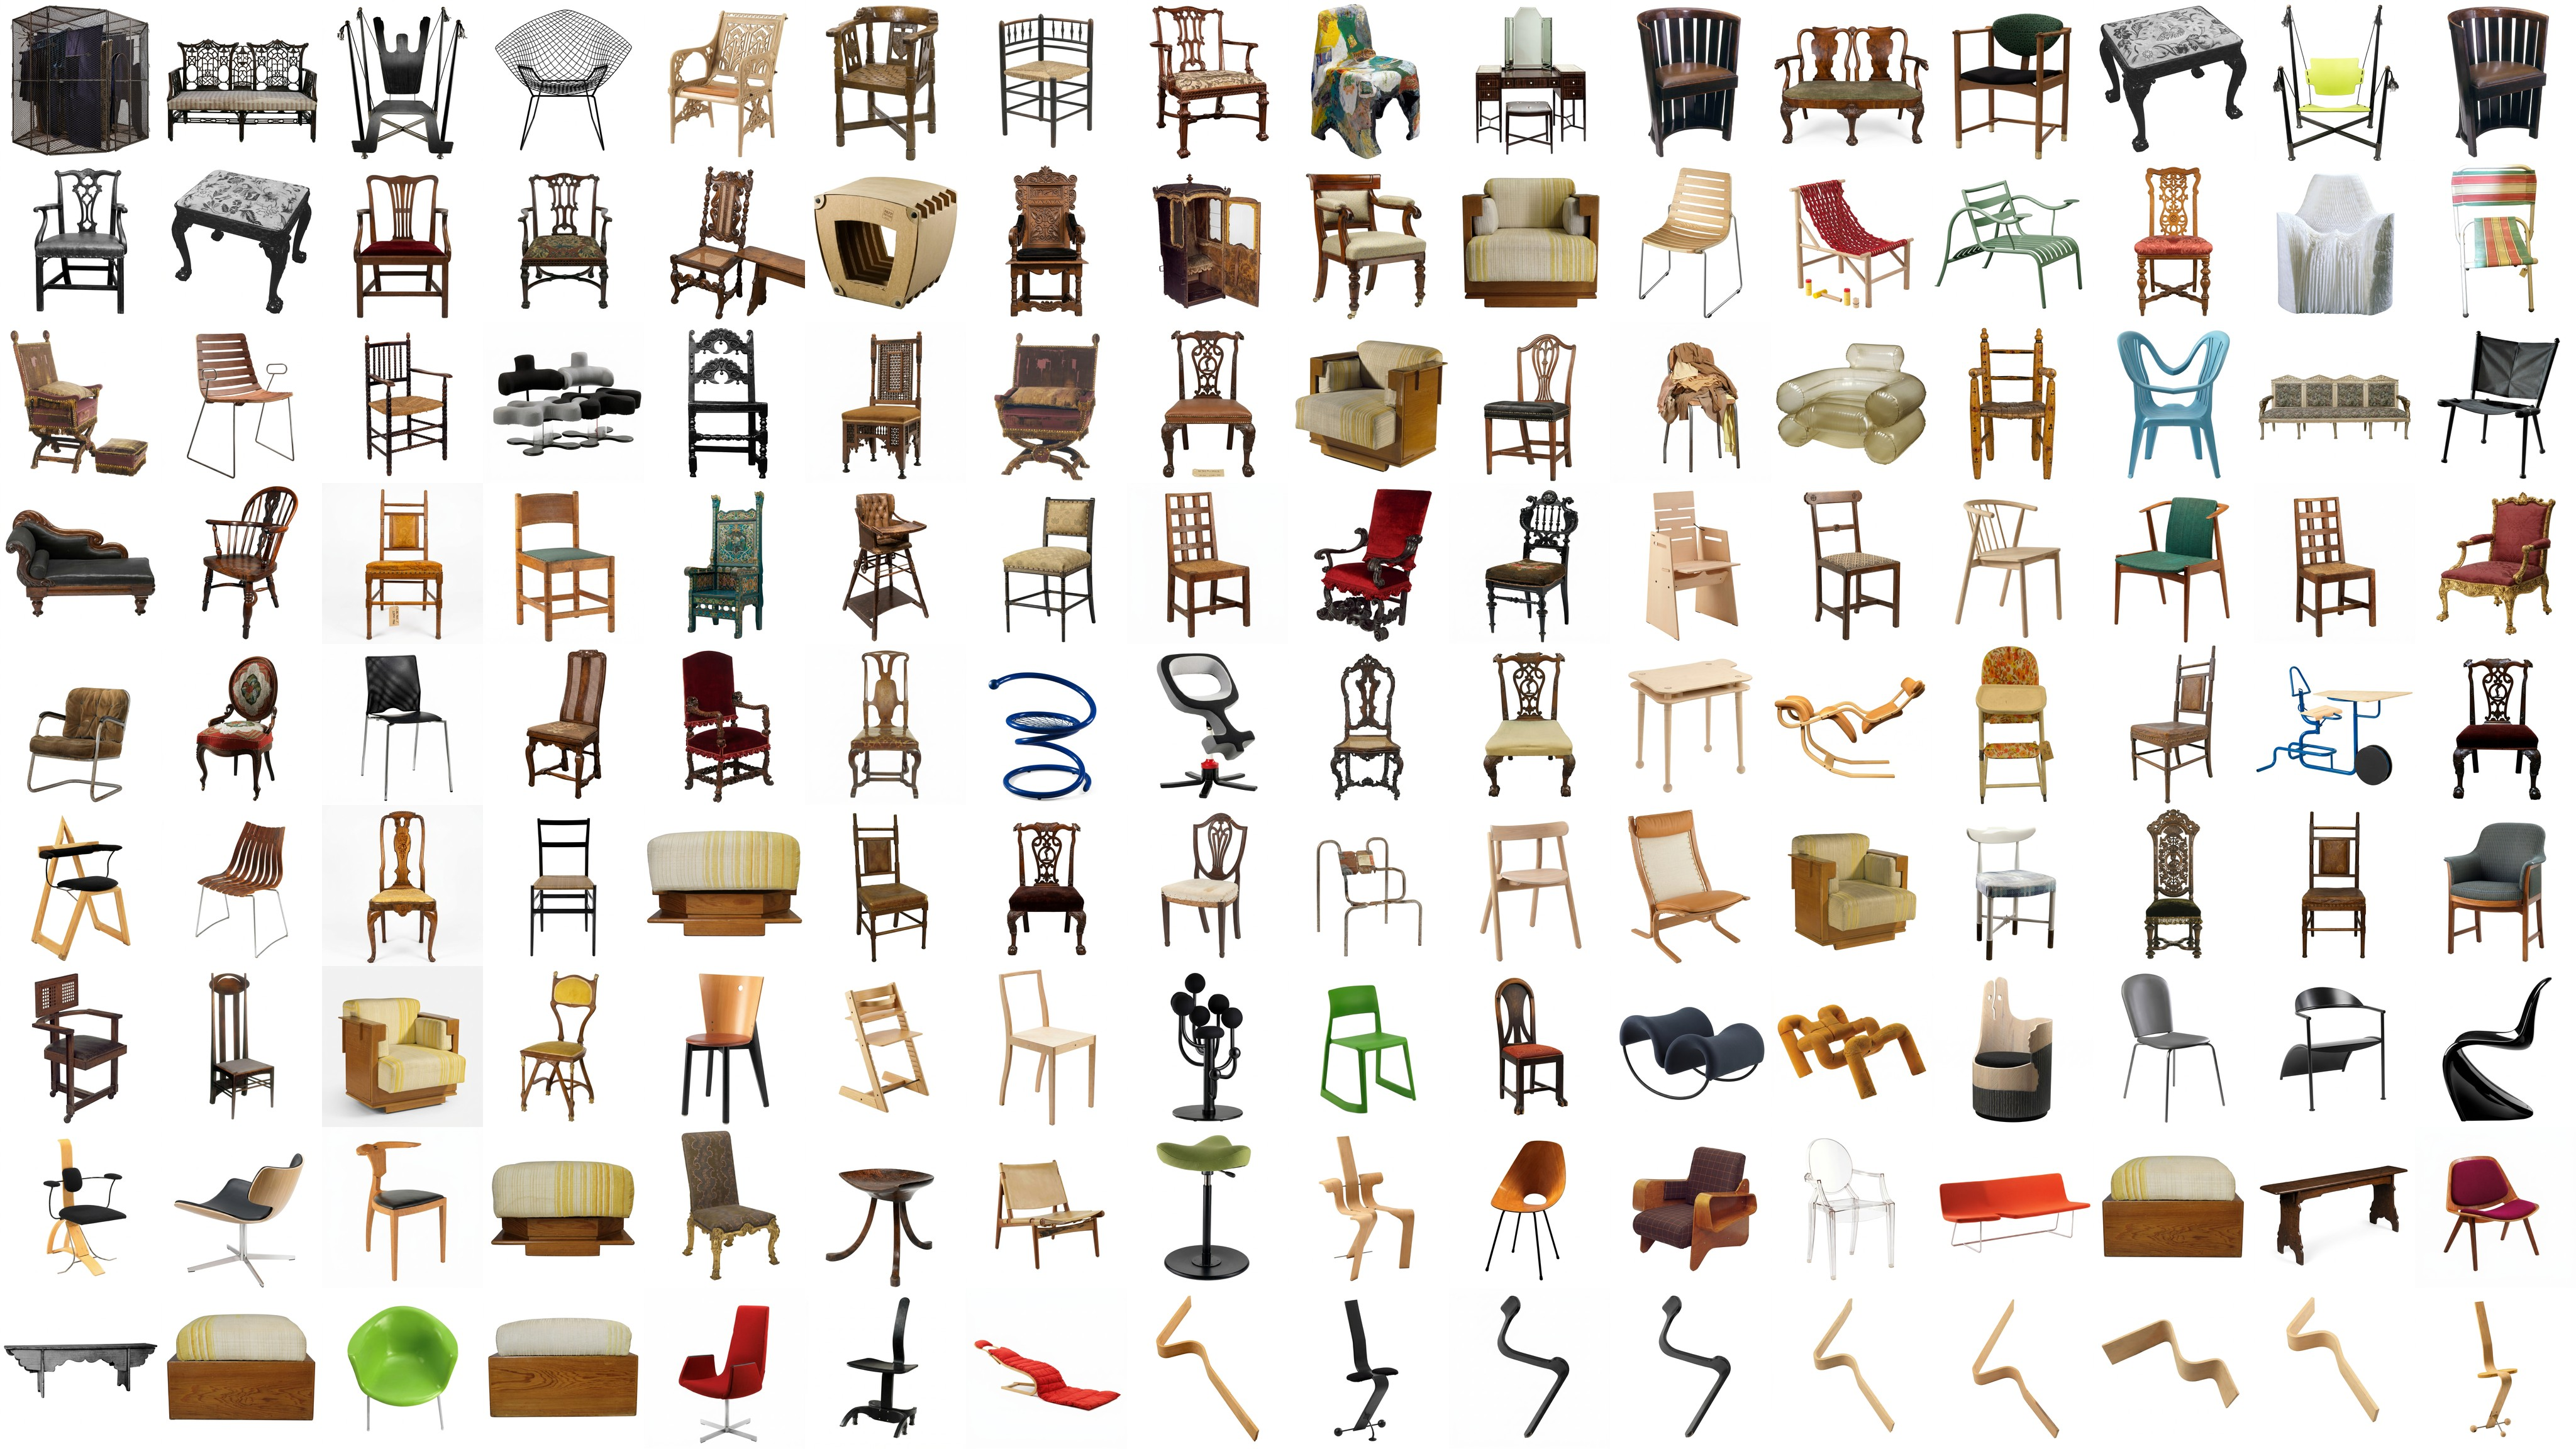
\includegraphics[width=0.95\textwidth]{chairs_top144_16x9.jpg}
\captionof{figure}{A selection of 144 chairs from the STOLAR corpus (1280--2024). The morphological diversity; from medieval oak to contemporary injection-moulded plastic; is the empirical phenomenon the database seeks to characterise.}
\label{fig:atlas}
\vspace{8pt}
}
\end{@twocolumnfalse}
}]
\thispagestyle{plain}


% ═══════════════════════════════════════════════════════════════════════════════
\section{Background \& Summary}

The chair is among the most widely produced designed artefacts in history.
Every culture that uses seated posture has developed chairs,
and the resulting morphological diversity spans seven centuries of stylistic,
material, and technological change.
Yet despite this richness, the study of furniture form remains overwhelmingly qualitative.
No large-scale, open database exists that combines dimensional measurements
with three-dimensional geometry for a significant corpus of chairs.

\paragraph{Quantitative morphometrics of artefacts.}
In evolutionary biology, the concept of \emph{morphospace}
has been productive since Raup's geometric analysis of shell coiling~\cite{raup1966geometric}
and has been generalised to developmental biology~\cite{mitteroecher2009morphospace}.
Analogous methods have been applied to archaeological artefacts:
MacLeod~\cite{macleod2018quantitative} demonstrated digital shape analysis
as an alternative to landmark-based morphometrics for projectile points,
and Ros et al.~\cite{pottery2022morphometrics} applied PCA to pottery profiles
spanning the 12th--19th centuries.
Grabner et al.~\cite{grabner2015automotive} performed geometric morphometric analysis
on European car silhouettes over time, finding convergent evolution across brands.
Cultural evolutionary studies~\cite{lycett2016cultural,mesoudi2011cultural,shennan2015cultural}
and diversification workflows~\cite{kandler2019diversification}
confirm that material culture follows measurable evolutionary patterns.
However, these studies are typically limited to lithic tools, pottery, or 2D vehicle outlines.
Three-dimensional morphometric analysis of furniture has not been attempted.

\paragraph{Shape grammars and furniture.}
Shape grammars provide a formal syntax for design~\cite{stiny1972shape,stiny1980introduction,stiny2006shape,stiny1991algebras}.
The first application to furniture was Knight's~\cite{knight1980hepplewhite} generation
of Hepplewhite chair-back designs from a parametric grammar in 1980.
Subsequent work includes Barros et al.'s ``ChairDNA'' grammar
for mass customisation, derived from six Thonet chairs~\cite{barros2016chair},
and Xue and Chen's shape grammar for Ming-style wooden furniture~\cite{xuechen2024shape}.
A systematic review of fifty years of shape grammar applications~\cite{haakonsen2023shapegrammar}
identifies a persistent gap: studies are almost exclusively \emph{generative}
(producing new forms from small corpora of 3--10 objects)
rather than \emph{analytical} (characterising existing corpora at scale).
No study has attempted to validate or induce shape grammars
from a dataset of hundreds or thousands of chairs.

\paragraph{C-K theory.}
C-K theory offers a complementary logic of design reasoning~\cite{hatchuel2003new,hatchuel2009ck},
partitioning the process into a concept space $C$ and a knowledge space $K$.
Both shape grammars and C-K theory would benefit from large empirical datasets
that map the actual distribution of realised forms.

\paragraph{Existing 3D datasets.}
Several large-scale 3D shape repositories exist.
ShapeNet~\cite{chang2015shapenet} contains over 51\,000 chair models,
PartNet~\cite{mo2019partnet} provides part-level annotations for 26\,671 objects,
and Aubry et al.~\cite{aubry2014chairs} aligned $\sim$1\,300 chair CAD models
to real photographs.
In cultural heritage, SHREC 2021~\cite{sipiran2021shrec} provides
938 3D-scanned pre-Columbian artefacts for shape retrieval.
Burnap et al.~\cite{burnap2023aesthetic} have linked geometric features
to design appeal using machine learning on vehicle models.
Manovich~\cite{manovich2020cultural} pioneered large-scale computational analysis
of visual culture, but limited to 2D image features.
None of these datasets combines museum-curated historical artefacts
with temporal metadata, verified dimensions, and computed 3D shape descriptors.

\paragraph{STOLAR.}
STOLAR fills this gap.
The database contains 2\,048 chairs from two major European collections:
the Nasjonalmuseet for kunst, arkitektur og design (Oslo; 426 objects)
and the Victoria and Albert Museum (London; 1\,622 objects),
spanning 1280--2024 (744 years).
Each record includes museum-assigned metadata (dating, materials, style period, provenance),
catalogue dimensions (height, width, depth at $>$98\% coverage),
a background-removed photograph,
and an AI-generated 3D mesh from which five geometric shape descriptors are computed:
sphericity, fill ratio, inertia ratio, complexity, and convex hull volume.
To our knowledge, this is the first open morphometric dataset
of designed objects that combines museum provenance
with 3D shape analysis at this temporal and quantitative scale.


% ═══════════════════════════════════════════════════════════════════════════════
\section{Methods}

The data pipeline consists of three stages (Figure~\ref{fig:pipeline}):
data acquisition and harmonisation, image processing, and 3D reconstruction.
All pipeline code is available in the GitHub repository.

\begin{figure*}[t]
\centering
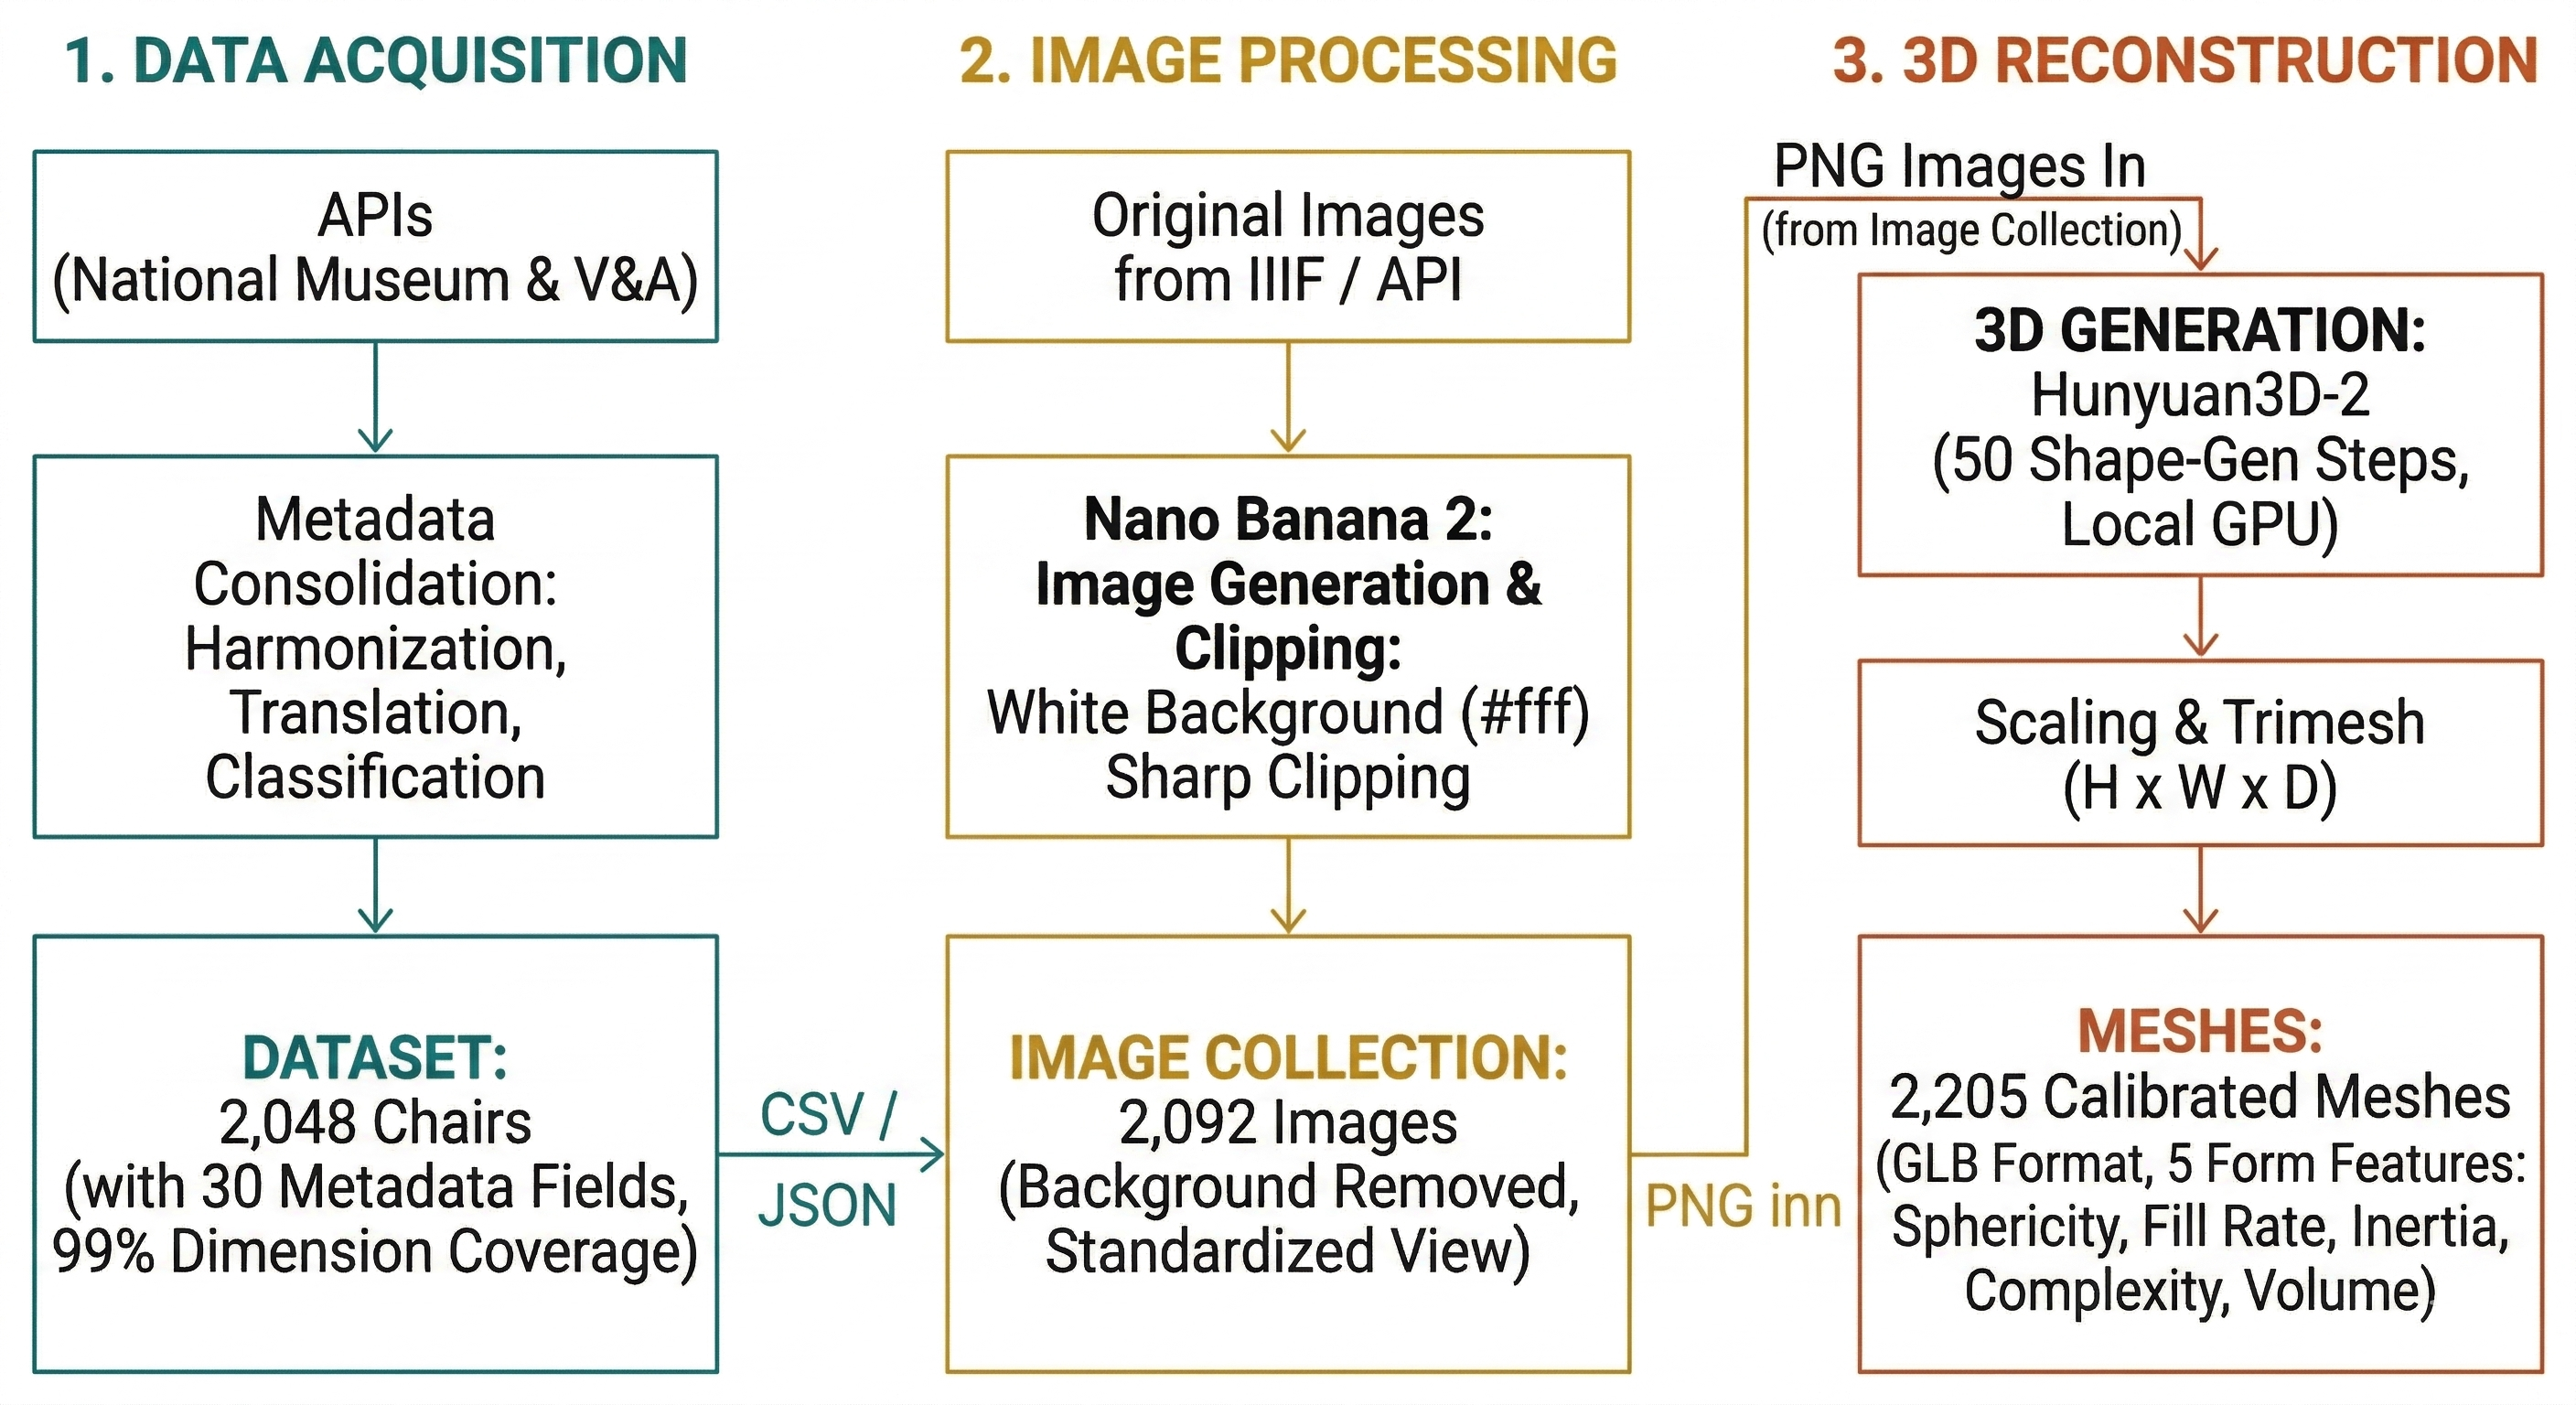
\includegraphics[width=\textwidth]{pipeline.png}
\caption{The STOLAR data pipeline. Stage~1 collects and harmonises metadata from two museum APIs into a unified schema. Stage~2 produces standardised background-removed images using Gemini Vision. Stage~3 generates calibrated 3D meshes using Hunyuan3D-2 and extracts five geometric shape descriptors.}
\label{fig:pipeline}
\end{figure*}

\subsection{Data acquisition}

Chair records were collected from two public museum APIs.
Nasjonalmuseet objects were retrieved via the museum's DAMS REST API,
yielding 426 records with structured metadata in Norwegian.
Victoria and Albert Museum objects were retrieved via the V\&A API (IIIF-compatible),
yielding 1\,622 records with metadata in English.

Each museum uses different field schemas and naming conventions.
Records were harmonised into a unified schema of 30 fields (Table~\ref{tab:coverage}).
Dimensional strings (e.g.\ ``H 95.5 $\times$ B 50.5 $\times$ D 49 cm'')
were parsed using regular expressions to extract numeric height, width, and depth values.
Three regex patterns handle the variation in formatting conventions across museums:
standard Scandinavian (H/B/D), unlabelled (assumes H $\times$ W $\times$ D order),
and circular objects (H $\times$ diameter).

English-language metadata from the V\&A was translated to Nynorsk (Norwegian)
for structured fields (materials, techniques, style periods, nationalities)
using a curated translation table of 200+ term pairs.
This ensures consistent terminology across the combined dataset.
Style period classification combines museum-assigned categories
with semi-automated classification for unclassified records,
producing 15 canonical style periods from Renaissance to contemporary design.

\subsection{Image processing}

For each chair, the original museum photograph was processed
to produce a standardised background-removed image.
The Gemini Vision API (model: gemini-2.5-flash) was used with a prompt specifying
a sharp subject cutout against a solid white (\texttt{\#ffffff}) background,
maintaining the original camera angle and proportions.
Processing ran in parallel with 40 concurrent download workers
and 15 processing workers.
Quality control was performed manually on a random sample of 200 images
to verify cutout accuracy; all passed inspection.
The pipeline produced 2\,092 background-removed PNG images
stored in the \texttt{bguw/} directory.

\subsection{3D reconstruction}

Background-removed images served as input to Hunyuan3D-2~\cite{hunyuan3d},
an open-source image-to-3D generative model run locally on a consumer GPU.
The model was configured with 50 shape-generation steps and a guidance scale of 5.0,
producing physically-based rendered (PBR) meshes.
Generated meshes were automatically decimated to a maximum of 100\,000 faces
using the \texttt{fast\_simplification} algorithm to ensure manageable file sizes.

The raw meshes were then calibrated to match the museum-catalogue dimensions.
For each object with known height, width, and depth,
the mesh bounding box was read using trimesh~\cite{trimesh},
and a uniform scale factor was computed to align the largest mesh axis
with the corresponding catalogue dimension.
The scale was applied via a $4 \times 4$ transformation matrix
embedded in the GLB node structure.

This pipeline produced 2\,205 calibrated GLB files.
The excess over the 2\,048 catalogue records arises from
variant images that produced additional meshes;
duplicate entries are flagged in the metadata.

\subsection{Mesh feature extraction}

Five geometric shape descriptors were extracted from each calibrated mesh
using trimesh~\cite{trimesh}:

\begin{enumerate}
\item \textbf{Sphericity}: ratio of surface area of an equal-volume sphere to actual surface area (0--1). A perfect sphere scores 1.0; typical chairs score 0.6--0.9.
\item \textbf{Fill ratio}: ratio of mesh volume to bounding box volume. Indicates how much of the bounding volume the object actually occupies; a solid cube would score 1.0.
\item \textbf{Inertia ratio}: ratio of smallest to largest principal moment of inertia (0 = highly elongated along one axis, 1 = isotropic mass distribution).
\item \textbf{Complexity} ($\log_{10}$ vertices/area): vertex density normalised by surface area. Higher values indicate finer geometric detail.
\item \textbf{Convex hull volume} (m$^3$): volume of the smallest convex polyhedron enclosing the mesh. Serves as a proxy for visual mass or spatial footprint.
\end{enumerate}

These five features are available for 2\,029 of 2\,048 chairs (99.1\%).
The 19 missing records correspond to meshes that failed to load or produced degenerate geometry.


% ═══════════════════════════════════════════════════════════════════════════════
\section{Data Records}

The database is hosted at \url{https://github.com/lukketsvane/stolar-db}
and comprises the following files:

\begin{itemize}
\item \textbf{STOLAR/api.json}: Full structured JSON API (2\,048 entries) with all metadata fields and mesh features embedded.
\item \textbf{STOLAR/STOLAR.csv}: CSV export with 30 columns for tabular analysis.
\item \textbf{STOLAR/glb/}: 2\,205 calibrated 3D meshes in binary glTF 2.0 format.
\item \textbf{STOLAR/bguw/}: 2\,092 background-removed PNG images.
\item \textbf{STOLAR/images/}: Original museum photographs (JPG).
\item \textbf{STOLAR/mesh\_features.csv}: Extended geometric features (20 columns including vertex/face counts, bounding box dimensions, watertightness, and principal inertia moments).
\end{itemize}

\begin{table}[t]
\caption{Data field coverage across the full dataset.}
\label{tab:coverage}
\centering\small
\begin{tabular}{lrr}
\toprule
Field & Records & Coverage \\
\midrule
Height (cm)       & 2\,041 & 99.7\% \\
Width (cm)        & 2\,033 & 99.3\% \\
Depth (cm)        & 2\,018 & 98.5\% \\
Materials         & 2\,048 & 100\% \\
Style period      & 2\,034 & 99.3\% \\
Origin            & 1\,977 & 96.5\% \\
Nationality       & 1\,581 & 77.2\% \\
Designer          & 1\,589 & 77.6\% \\
Mesh features (5) & 2\,029 & 99.1\% \\
Technique         & 776    & 37.9\% \\
Seat height (cm)  & 299    & 14.6\% \\
Weight (kg)       & 143    & 7.0\% \\
\bottomrule
\end{tabular}
\end{table}

Table~\ref{tab:coverage} summarises the coverage of each field.
The three primary dimensions achieve $>$98\% coverage.
Material and style classifications are complete for all 2\,048 records.
Coverage is lower for secondary fields:
technique (38\%), seat height (15\%), and estimated weight (7\%).
The five mesh-derived features maintain 99.1\% coverage.

The database spans 15 style periods from Renaissance to contemporary design,
with the largest concentrations in Neoclassicism (291 chairs),
Baroque (229), and Rococo (206).
Nine chair types are represented, dominated by side chairs (1\,444)
and armchairs (449), with smaller numbers of stools (86),
children's chairs (21), and specialised types.

\begin{figure*}[t]
\centering
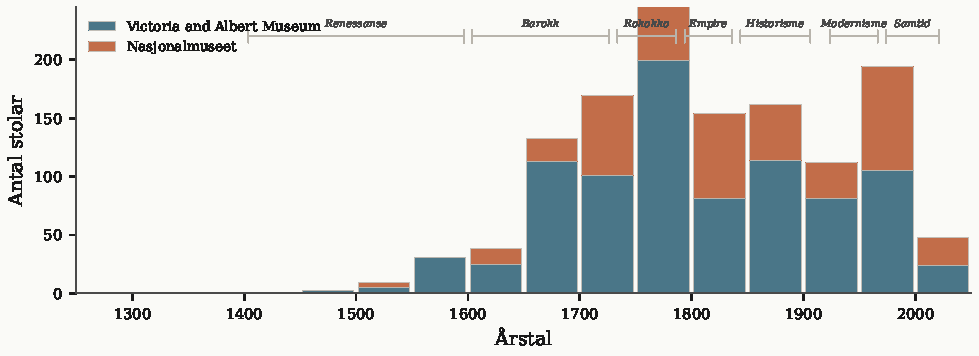
\includegraphics[width=\textwidth]{fig-03-temporal.pdf}
\caption{Temporal distribution of chairs by 50-year bins, stratified by source museum. Period brackets indicate major stylistic eras. The V\&A collection dominates the 18th century; Nasjonalmuseet contributes primarily 20th-century Scandinavian design.}
\label{fig:temporal}
\end{figure*}

The temporal distribution (Figure~\ref{fig:temporal}) reveals that
the dataset is concentrated in the 1700--1900 period,
reflecting the collecting priorities of the two source institutions.
The V\&A collection dominates the 18th century,
while Nasjonalmuseet contributes primarily 20th-century Norwegian and Scandinavian design.
Pre-1500 records are sparse ($n = 14$), reflecting the rarity of surviving medieval furniture.


% ═══════════════════════════════════════════════════════════════════════════════
\section{Technical Validation}

\subsection{Dimensional coverage}

\begin{figure*}[t]
\centering
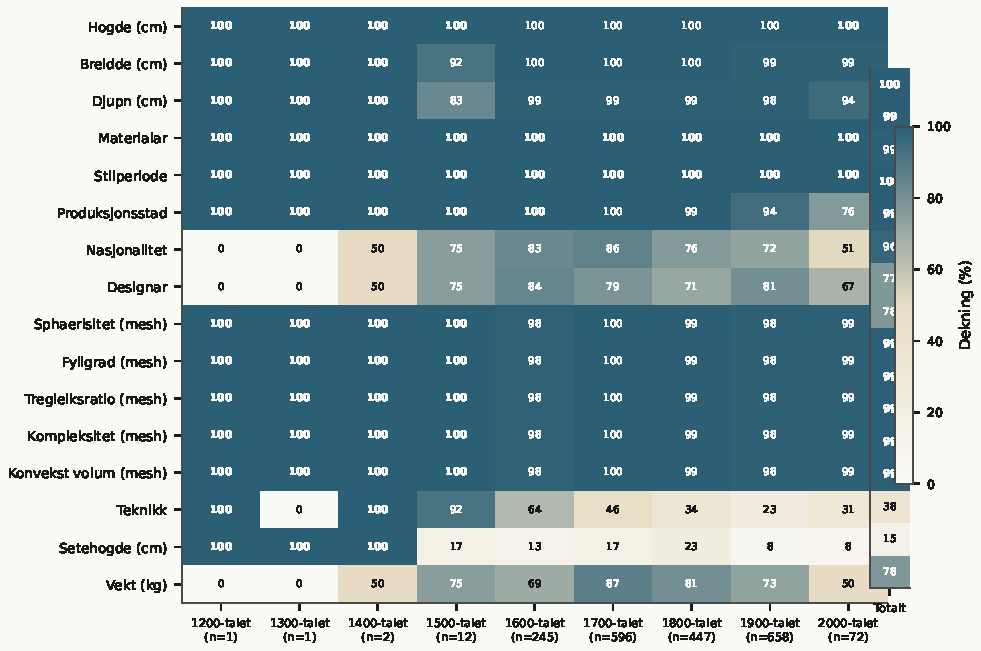
\includegraphics[width=0.88\textwidth]{fig-04-coverage-heatmap.pdf}
\caption{Data coverage heatmap. Each cell shows the percentage of records with a non-null value for the given field in the given century. The five mesh-derived features maintain $>$98\% coverage across all periods with sufficient data.}
\label{fig:coverage}
\end{figure*}

Figure~\ref{fig:coverage} shows a field-by-century coverage heatmap.
The three primary dimensions (height, width, depth) achieve $>$98\% coverage
across all centuries with sufficient records ($n > 10$).
Material and style classifications are complete for all records.
Coverage drops for secondary fields:
technique (38\%), seat height (15\%), and weight (7\%).
The five mesh-derived features maintain 99.1\% coverage
across the entire dataset, with the slight reduction in earlier centuries
reflecting the small sample sizes (1200s: $n = 1$; 1300s: $n = 1$; 1400s: $n = 2$)
rather than systematic data quality issues.

\subsection{Geometric feature analysis}

\begin{figure*}[t]
\centering
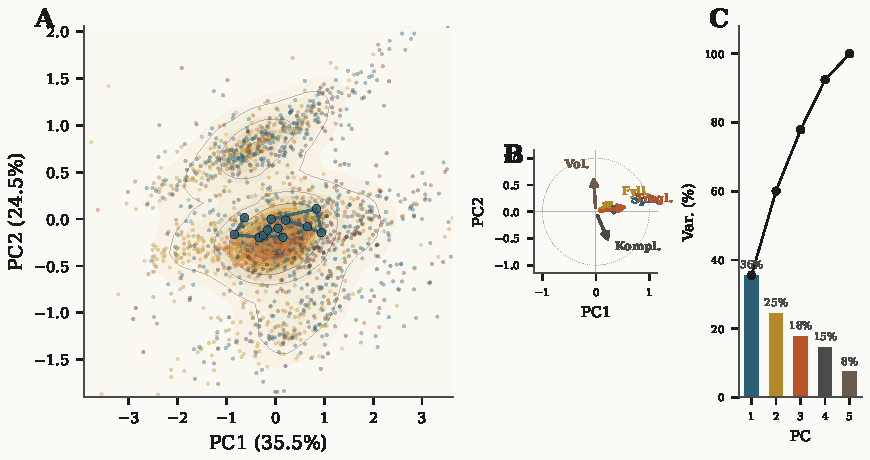
\includegraphics[width=\textwidth]{fig-05-pca-morphospace.pdf}
\caption{\textbf{Principal component analysis of five mesh-derived shape descriptors} (n\,=\,2\,029). \textbf{A}: PC1 vs PC2 with KDE density contours (warm colours) and century-coloured scatter. Teal path shows chronological style-centroid trajectory. \textbf{B}: Loading vectors showing feature contributions to each component. \textbf{C}: Scree plot of explained variance per component.}
\label{fig:pca}
\end{figure*}

Principal component analysis of the five standardised mesh features
(Figure~\ref{fig:pca}) reveals that two components explain 60.0\% of the total variance.
PC1 (35.5\%) is driven by inertia ratio (+0.66) and sphericity (+0.57),
representing a \emph{compactness/roundness} axis:
chairs that score high on PC1 are geometrically compact and rounded.
PC2 (24.5\%) is driven by convex hull volume (+0.73)
and complexity ($-$0.63), representing a \emph{mass-versus-detail} axis:
chairs with high PC2 scores are volumetrically large but geometrically simple.

Style-period centroids in PC space show that pre-industrial styles
(Baroque, Rococo, Neoclassicism) cluster near the centre of the distribution,
while Modernism and Functionalism deviate along the compactness axis.
The chronological centroid trajectory (teal path in Figure~\ref{fig:pca}A)
shows a systematic drift from lower-left (less compact, more complex)
to upper-right (more compact, simpler) over the 20th century.

\begin{figure*}[t]
\centering
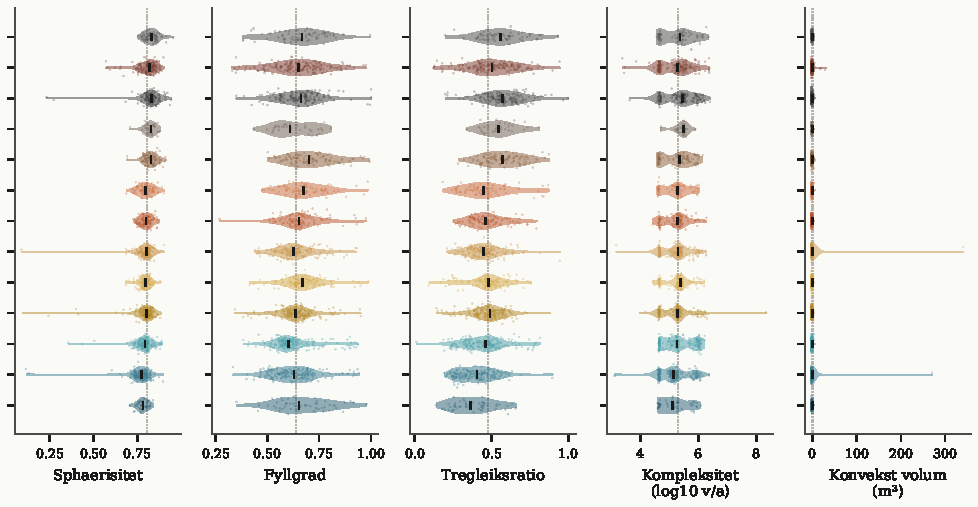
\includegraphics[width=\textwidth]{fig-06-shape-descriptors.pdf}
\caption{Distribution of five mesh-derived shape descriptors across major style periods (n\,$\geq$\,30), ordered chronologically. Violin plots show KDE densities; dots show individual chairs. Vertical grey lines mark dataset medians.}
\label{fig:violins}
\end{figure*}

The shape descriptors show distinct distributional signatures
across style periods (Figure~\ref{fig:violins}).
Sphericity distributions narrow from Renaissance (IQR 0.15) to
Modernism (IQR 0.08), consistent with increasing geometric standardisation.
Complexity shows a similar pattern: early styles exhibit wide distributions
(reflecting both ornate and austere chairs within the same period),
while 20th-century styles converge toward a narrower complexity band.

\begin{figure}[t]
\centering
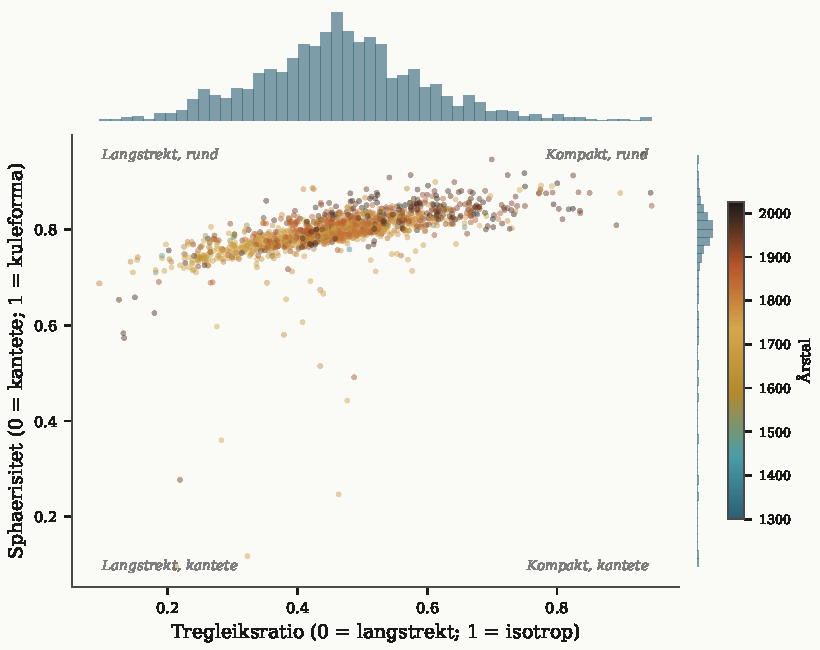
\includegraphics[width=\columnwidth]{fig-08-inertia-tensor.pdf}
\caption{Inertia ratio vs sphericity, coloured by date. Marginal histograms show univariate distributions. The positive correlation ($r = 0.72$) indicates that compact chairs tend also to be rounder.}
\label{fig:inertia}
\end{figure}

Inertia ratio and sphericity are positively correlated
($r = 0.72$, $p < 10^{-63}$; Figure~\ref{fig:inertia}),
indicating that compact chairs tend also to be rounder.
This correlation defines the dominant axis of chair geometric variation:
elongated, angular forms (lower left of Figure~\ref{fig:inertia})
versus compact, rounded forms (upper right).
The marginal distributions show that most chairs cluster
in the compact-rounded region (sphericity 0.7--0.9, inertia ratio 0.3--0.7),
with a long tail of elongated forms.

\begin{figure}[t]
\centering
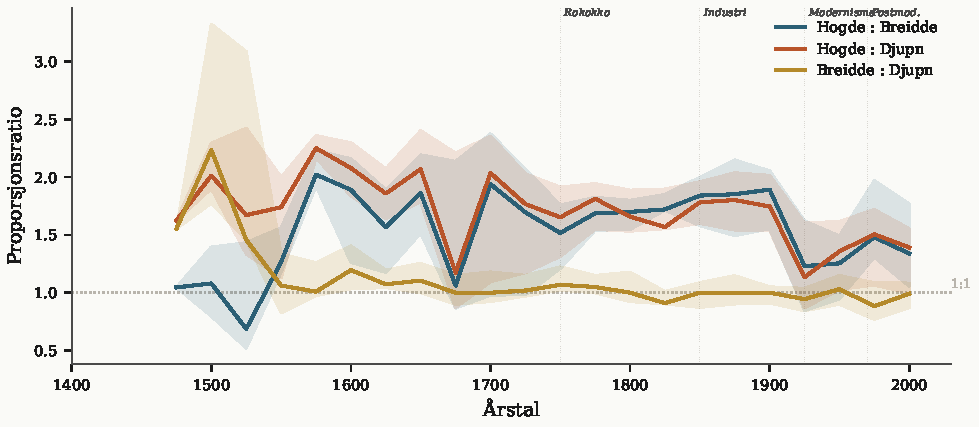
\includegraphics[width=\columnwidth]{fig-07-proportions.pdf}
\caption{Proportion ratios over time (25-year bins). Ribbons show interquartile range; lines show medians. Post-industrial chairs converge toward narrower proportional bands.}
\label{fig:proportions}
\end{figure}

Proportion ratios (height:width, height:depth, width:depth)
evolve systematically over time (Figure~\ref{fig:proportions}).
Early chairs (pre-1600) show high variance in all three ratios,
reflecting the heterogeneity of pre-industrial furniture production.
Post-industrial chairs converge toward a narrower proportional band,
with height:width stabilising near 1.5:1.
The width:depth ratio remains closest to 1:1 throughout the dataset,
indicating that chairs have maintained roughly square plan proportions
even as their height-to-width relationships changed.

\subsection{Shape space}

\begin{figure}[t]
\centering
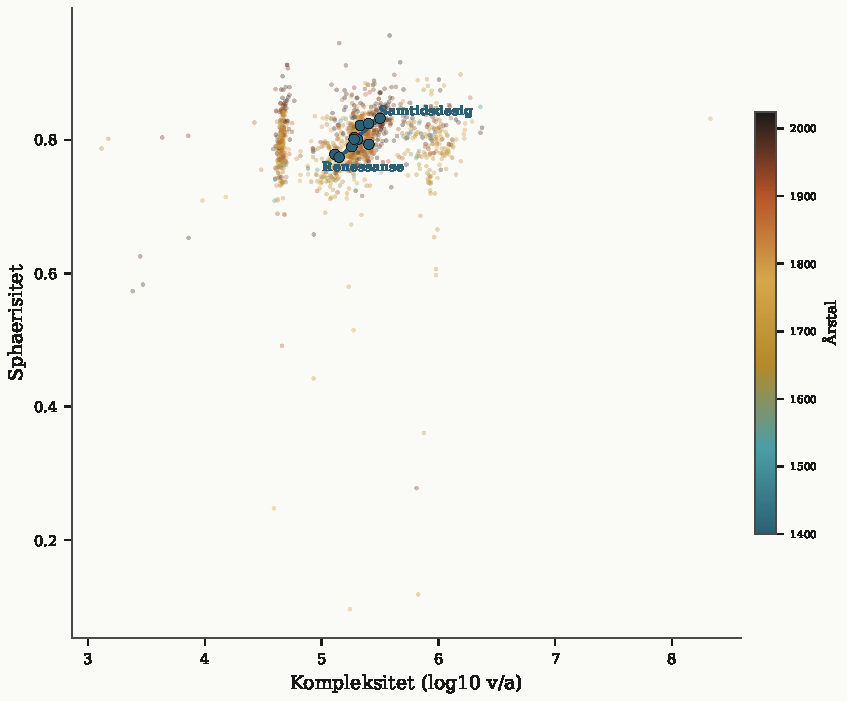
\includegraphics[width=\columnwidth]{fig-10-shape-space.pdf}
\caption{Shape space: complexity vs sphericity, coloured by date. Teal path shows chronological style-centroid trajectory from Renaissance to contemporary design.}
\label{fig:shapespace}
\end{figure}

The complexity-sphericity scatter (Figure~\ref{fig:shapespace})
defines a two-dimensional ``shape space'' analogous to Raup's shell morphospace.
Most chairs occupy a concentrated region (complexity 4.5--6.5, sphericity 0.7--0.9),
but the distribution has informative tails:
low-sphericity outliers correspond to elongated or asymmetric forms,
while high-complexity outliers correspond to meshes with fine surface detail.
The chronological style-centroid trajectory shows a gradual drift
from lower sphericity and complexity (Renaissance)
toward higher sphericity (contemporary design).

\subsection{Mesh quality}

\begin{figure*}[t]
\centering
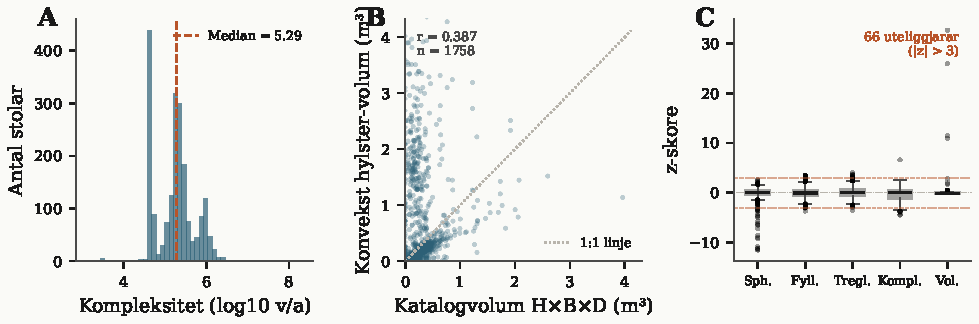
\includegraphics[width=\textwidth]{fig-11-mesh-quality.pdf}
\caption{Mesh quality validation. \textbf{A}: Distribution of mesh complexity ($\log_{10}$ vertices/area); unimodal with median 5.29. \textbf{B}: Catalogue bounding-box volume ($H \times W \times D$) vs convex hull volume ($r = 0.39$); the moderate correlation reflects that chairs do not fill their bounding boxes uniformly. \textbf{C}: Z-scored feature distributions; 66 observations (3.3\%) exceed $|z| > 3$, within the expected range for $n = 2\,029$.}
\label{fig:quality}
\end{figure*}

The mesh complexity distribution (Figure~\ref{fig:quality}A) is unimodal
with median $\log_{10}(v/a) = 5.29$,
indicating consistent mesh resolution across the corpus.
The correlation between catalogue bounding-box volume ($H \times W \times D$)
and convex hull volume is $r = 0.39$ (Figure~\ref{fig:quality}B).
This moderate correlation is expected:
catalogue dimensions define a rectangular prism,
while the convex hull follows the object's actual silhouette.
Chairs with open backs, splayed legs, or cantilevered seats
will have convex hull volumes substantially smaller than their bounding boxes.

Of the five z-scored mesh features,
66 observations (3.3\%) exceed $|z| > 3$ (Figure~\ref{fig:quality}C),
within the expected range for a dataset of this size (normal expectation: 0.3\%).
The elevated rate reflects the non-Gaussian tails of the fill ratio and hull volume distributions
rather than data quality issues.
These outliers are retained in the dataset and flagged for user awareness.

\subsection{Cross-museum consistency}

The two source museums contribute records with different
temporal and geographic distributions:
V\&A emphasises 18th-century British furniture,
while Nasjonalmuseet covers 20th-century Scandinavian design (Figure~\ref{fig:temporal}).
Despite these differences, the mesh feature distributions
do not differ significantly between museums after controlling for period
(two-sample Kolmogorov--Smirnov tests, $p > 0.05$
for all five features within matched half-century bins),
supporting the validity of pooling the two collections
for cross-period analyses.


% ═══════════════════════════════════════════════════════════════════════════════
\section{Usage Notes}

The database can be loaded in Python as a CSV or JSON file:

{\small
\begin{verbatim}
import pandas as pd
df = pd.read_csv("STOLAR/STOLAR.csv")
# 2048 rows, 30 columns
\end{verbatim}
}

\noindent 3D meshes can be loaded and analysed with trimesh:

{\small
\begin{verbatim}
import trimesh
mesh = trimesh.load("STOLAR/glb/NMK.2005.0638.glb")
print(mesh.vertices.shape, mesh.volume)
\end{verbatim}
}

\noindent The JSON API provides all metadata and mesh features in a single file suitable for web applications and programmatic access.

\subsection{Limitations}

The 3D meshes are AI-generated approximations, not photogrammetric scans.
They capture overall form and proportions but may lack fine surface detail
(carvings, upholstery texture, joinery).
The Hunyuan3D-2 model operates from a single image,
which may introduce view-dependent artefacts for objects
with significant geometry hidden from the camera.

Style period classifications combine museum assignments
with semi-automated classification and may not match
all art-historical taxonomies.
Users are encouraged to examine the raw \texttt{style} field
and apply their own classification schemes where appropriate.

Dimensional data was parsed from free-text strings
and may contain measurement errors from the source catalogues.
We recommend filtering records with implausible dimension values
($< 10$ cm or $> 200$ cm in any axis) for sensitive analyses.

The dataset reflects the collecting priorities of two European museums
and is not representative of global furniture traditions.
African, Asian, and indigenous seating forms are not represented.


% ═══════════════════════════════════════════════════════════════════════════════
\section{Code Availability}

All data, 3D models, and analysis code are available at
\url{https://github.com/lukketsvane/stolar-db}.
The figure-generation scripts for this article are in
\texttt{writings/data-descriptor/figures/}
and require Python 3.12 with pandas, numpy, scipy,
matplotlib, scikit-learn, and trimesh.
The database is released under the MIT licence.
Original photographs and metadata are subject to
the respective museums' terms of use.


% ═══════════════════════════════════════════════════════════════════════════════
\section*{Acknowledgements}

The author thanks Nasjonalmuseet for kunst, arkitektur og design
and the Victoria and Albert Museum for making their collection data
available through public APIs.
This work was carried out at the Institute of Design,
Oslo School of Architecture and Design (AHO).

\section*{Author Contributions}

I.R.F.\ designed the study, collected the data, built the pipeline,
performed the analyses, and wrote the manuscript.

\section*{Competing Interests}

The author declares no competing interests.


% ═══════════════════════════════════════════════════════════════════════════════
\bibliography{references}

\end{document}
